
\chapter[Planejamento do projeto]{Planejamento do projeto}


\section{\large{Cronograma}} 

\tab Para uma boa gestão do recursos, equipe e principalmente tempo, é necessária a criação de um cronograma para demonstrar de forma intuitiva e eficiente a programação das atividades do grupo. O cronograma a seguir demonstra o planejamento de atividades, duração, data de início, data de fim, responsável e grau de conclusão. A ferramenta escolhida foi o Gantter, visto que é online e que tem a opão de ser integrado com o Google Drive, permitindo a múltipla edição simultânea por diversos membros da equipe. \\

 


\begin{figure}[h]
	\centering
	\label{fig01}
		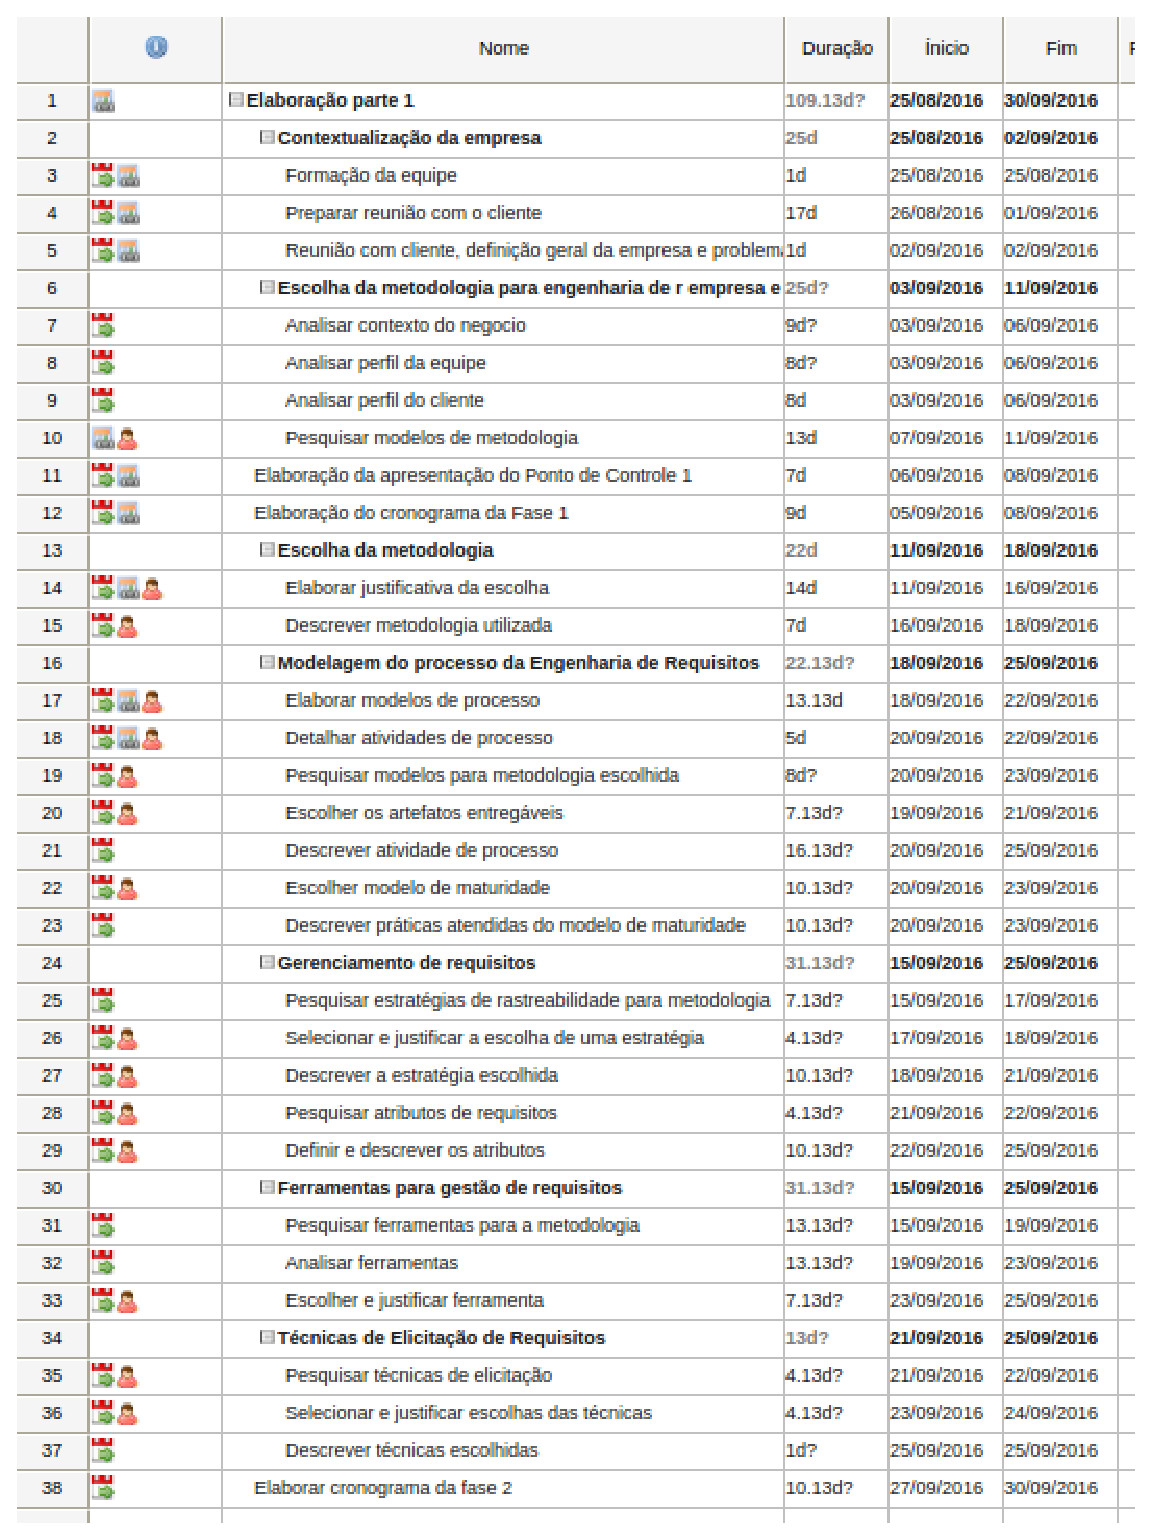
\includegraphics[keepaspectratio=true,scale=0.6]{figuras/cronogramamaior.eps}
	\caption{Cronograma do Projeto}
\end{figure}
